\documentclass{article}\usepackage{amsmath,amssymb,amsthm,tikz,tkz-graph,color,chngpage,soul,hyperref,csquotes,graphicx,floatrow,circuitikz}\newcommand*{\QEDB}{\hfill\ensuremath{\square}}\newtheorem*{prop}{Proposition}\renewcommand{\theenumi}{\alph{enumi}}\usepackage[shortlabels]{enumitem}\usepackage[nobreak=true]{mdframed}\usetikzlibrary{matrix,calc}\MakeOuterQuote{"}\usepackage[margin=0.75in]{geometry} \newtheorem{theorem}{Theorem}

\title{CS70 - Lecture 12 Notes}
\author{Name: Felix Su$\quad$SID: 25794773}
\date{Spring 2016$\quad$GSI: Gerald Zhang}
\begin{document}
\maketitle

%%%% Topic %%%%
\subsection*{Berklekamp-Welsh Algorithm}
%%%% Notes %%%%
\textbf{Existence:}
\begin{itemize}
\item Exists because packets constructed using $P(x)$
\end{itemize}
\textbf{Unique:}
\begin{itemize}
\item Proved assuming $\frac{Q'(x)}{E(x)} = \frac{Q(x)}{E'(x)} = P(x$
\item $E(x)$ and $E'(x)$ have at most $k$ roots each
\item Cross multiply assumption at $n$ valid points, so claim is true for $n$ points, which make $P(x)$ a unique $< n$ degree polynomial
\item \textbf{Fact:} $Q'(x)E(x) = Q(x)E'(x)$ on $n+2k$ values of $x$
    \begin{itemize}
        \item Holds when $E(x)$ or $E'(x)$ are 0
        \item Use above method of cross multiplication when not zero
    \end{itemize}
\end{itemize}
\begin{mdframed}
\textbf{Encoding/Decoding Polynomial Summary:}\\
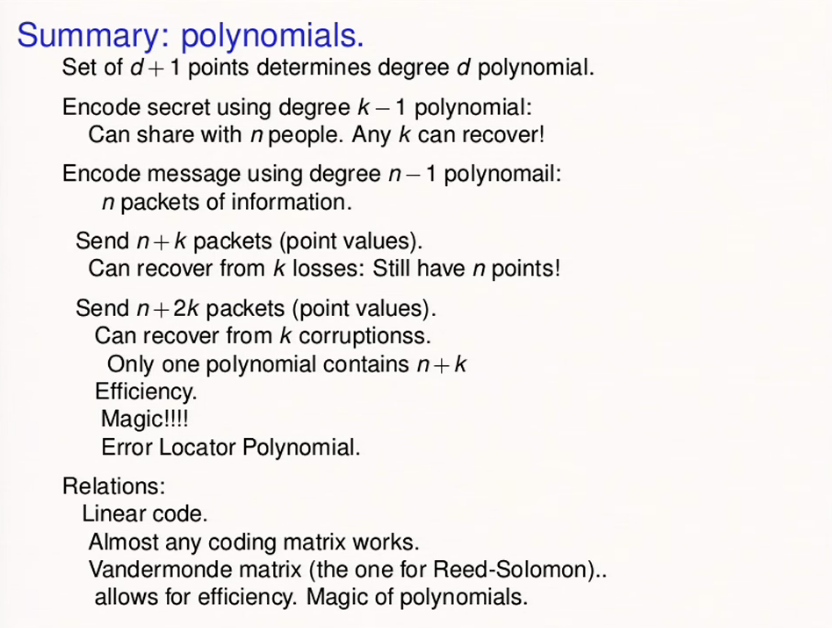
\includegraphics{polysum}
\end{mdframed}

%%%% Topic %%%%
\subsection*{Counting}
%%%% Notes %%%%
\begin{itemize}
    \item Counting Numbers: 0,1,2... all Natural Numbers $\mathbb{N}$
    \item \textbf{Countable if there is a bijection between $S$ and some subset of $\mathbb{N}$}
    \item if subset of $\mathbb{N}$ = finite, $S$ has finite \textbf{cardinality}
    \item if subset of $\mathbb{N}$ = infinite, $S$ is \textbf{countably infinite}
        \begin{itemize}
            \item Evens are countably infinite
            \item Integers are countably infinite
            \item Pairs of Natural Numbers are countably infinite
            \item Rationals are countably infinite (subset of pairs of natural numbers with gcd of 1)
            \item Reals are uncountable
        \end{itemize}
    \item All countably infinite sets have the same cardinality
\end{itemize}
\textbf{Isomorphism Principle:}
\begin{itemize}
    \item If there is $f: D\rightarrow R$ that is one to one and onto, (bijective) then $|D| = |R|$
\end{itemize}
\textbf{Listing:}
\begin{itemize}
    \item A bijection with a subset of natural numbers
    \item The $n$th item in the list is a mapping $n \in \mathbb{N} \rightarrow f(n)$
    \item If you can list a set you can show a bijection
    \item Finite List: Bijection with subset of $\mathbb{N}\{0, ..., |S|-1\}$
    \item Infinite List: Bijection with $\mathbb{N}$
\end{itemize}
\textbf{Enumerating $\equiv$ Countability =  Listing:}
\begin{itemize}
    \item Enumerating a set $\implies$ countability
    \item Corollary: Any subset $T$ of a countable set $S$ is also countable
    \item Each element of $x \in S$ has a specific, finite position in a list (ex. $\mathbb{Z} = \{0,1,-1,2,-2,...\}$
    \item Fails for integers if you list positive integers before negative integers
        \begin{itemize}
            \item $\mathbb{Z} = \{\{0,1,2,...,\}$ and then $\{-1,-2,...\}\}$
            \item -1s position is not finite, because there are $\infty$ positive integers
            \item So.. you must \textbf{interweave}
        \end{itemize}
\end{itemize}
\textbf{Diagonalization:}
\begin{itemize}
    \item \textbf{Diagonal Number} Number that is not in the list of $f(n)$
    \item Ex. Method to create diagonal number for Reals: Digit $i$ is 7 if number $i$'s $i$th digit is not 7, 6 otherwise. For every $n$th position on the list, at least the $n$th digit will be different than the diagonal number's $n$th digit. Contradiction because the diagonal number is real.
    \item Check if this creates contradicton. If diagonal number is in the questionable set, the list could not have existed and thes et is not countable.
\end{itemize}
\end{document}